\documentclass{report}
\usepackage{subcaption}
\usepackage{tocloft}
\usepackage{graphicx}
\usepackage{float}
\usepackage{hyperref}
\usepackage{biblatex}[style=ieeetr, sorting=none, backend=biber]
\usepackage[a4paper, left=15mm, right=15mm, top=15mm, bottom=15mm]{geometry}
\addbibresource{main.bib}
\author{QUT Aerospace Society}
\title{Technical Report: CubeSAT}
\setcounter{tocdepth}{3}
\begin{document}    
    \maketitle
    \tableofcontents
    \chapter{CubeSAT Overview}
    % high level overview of design of the payload system
    % design functinoality of the payload system
        \section{Technical Breakdown}
            \begin{figure}[H]
                \centering
                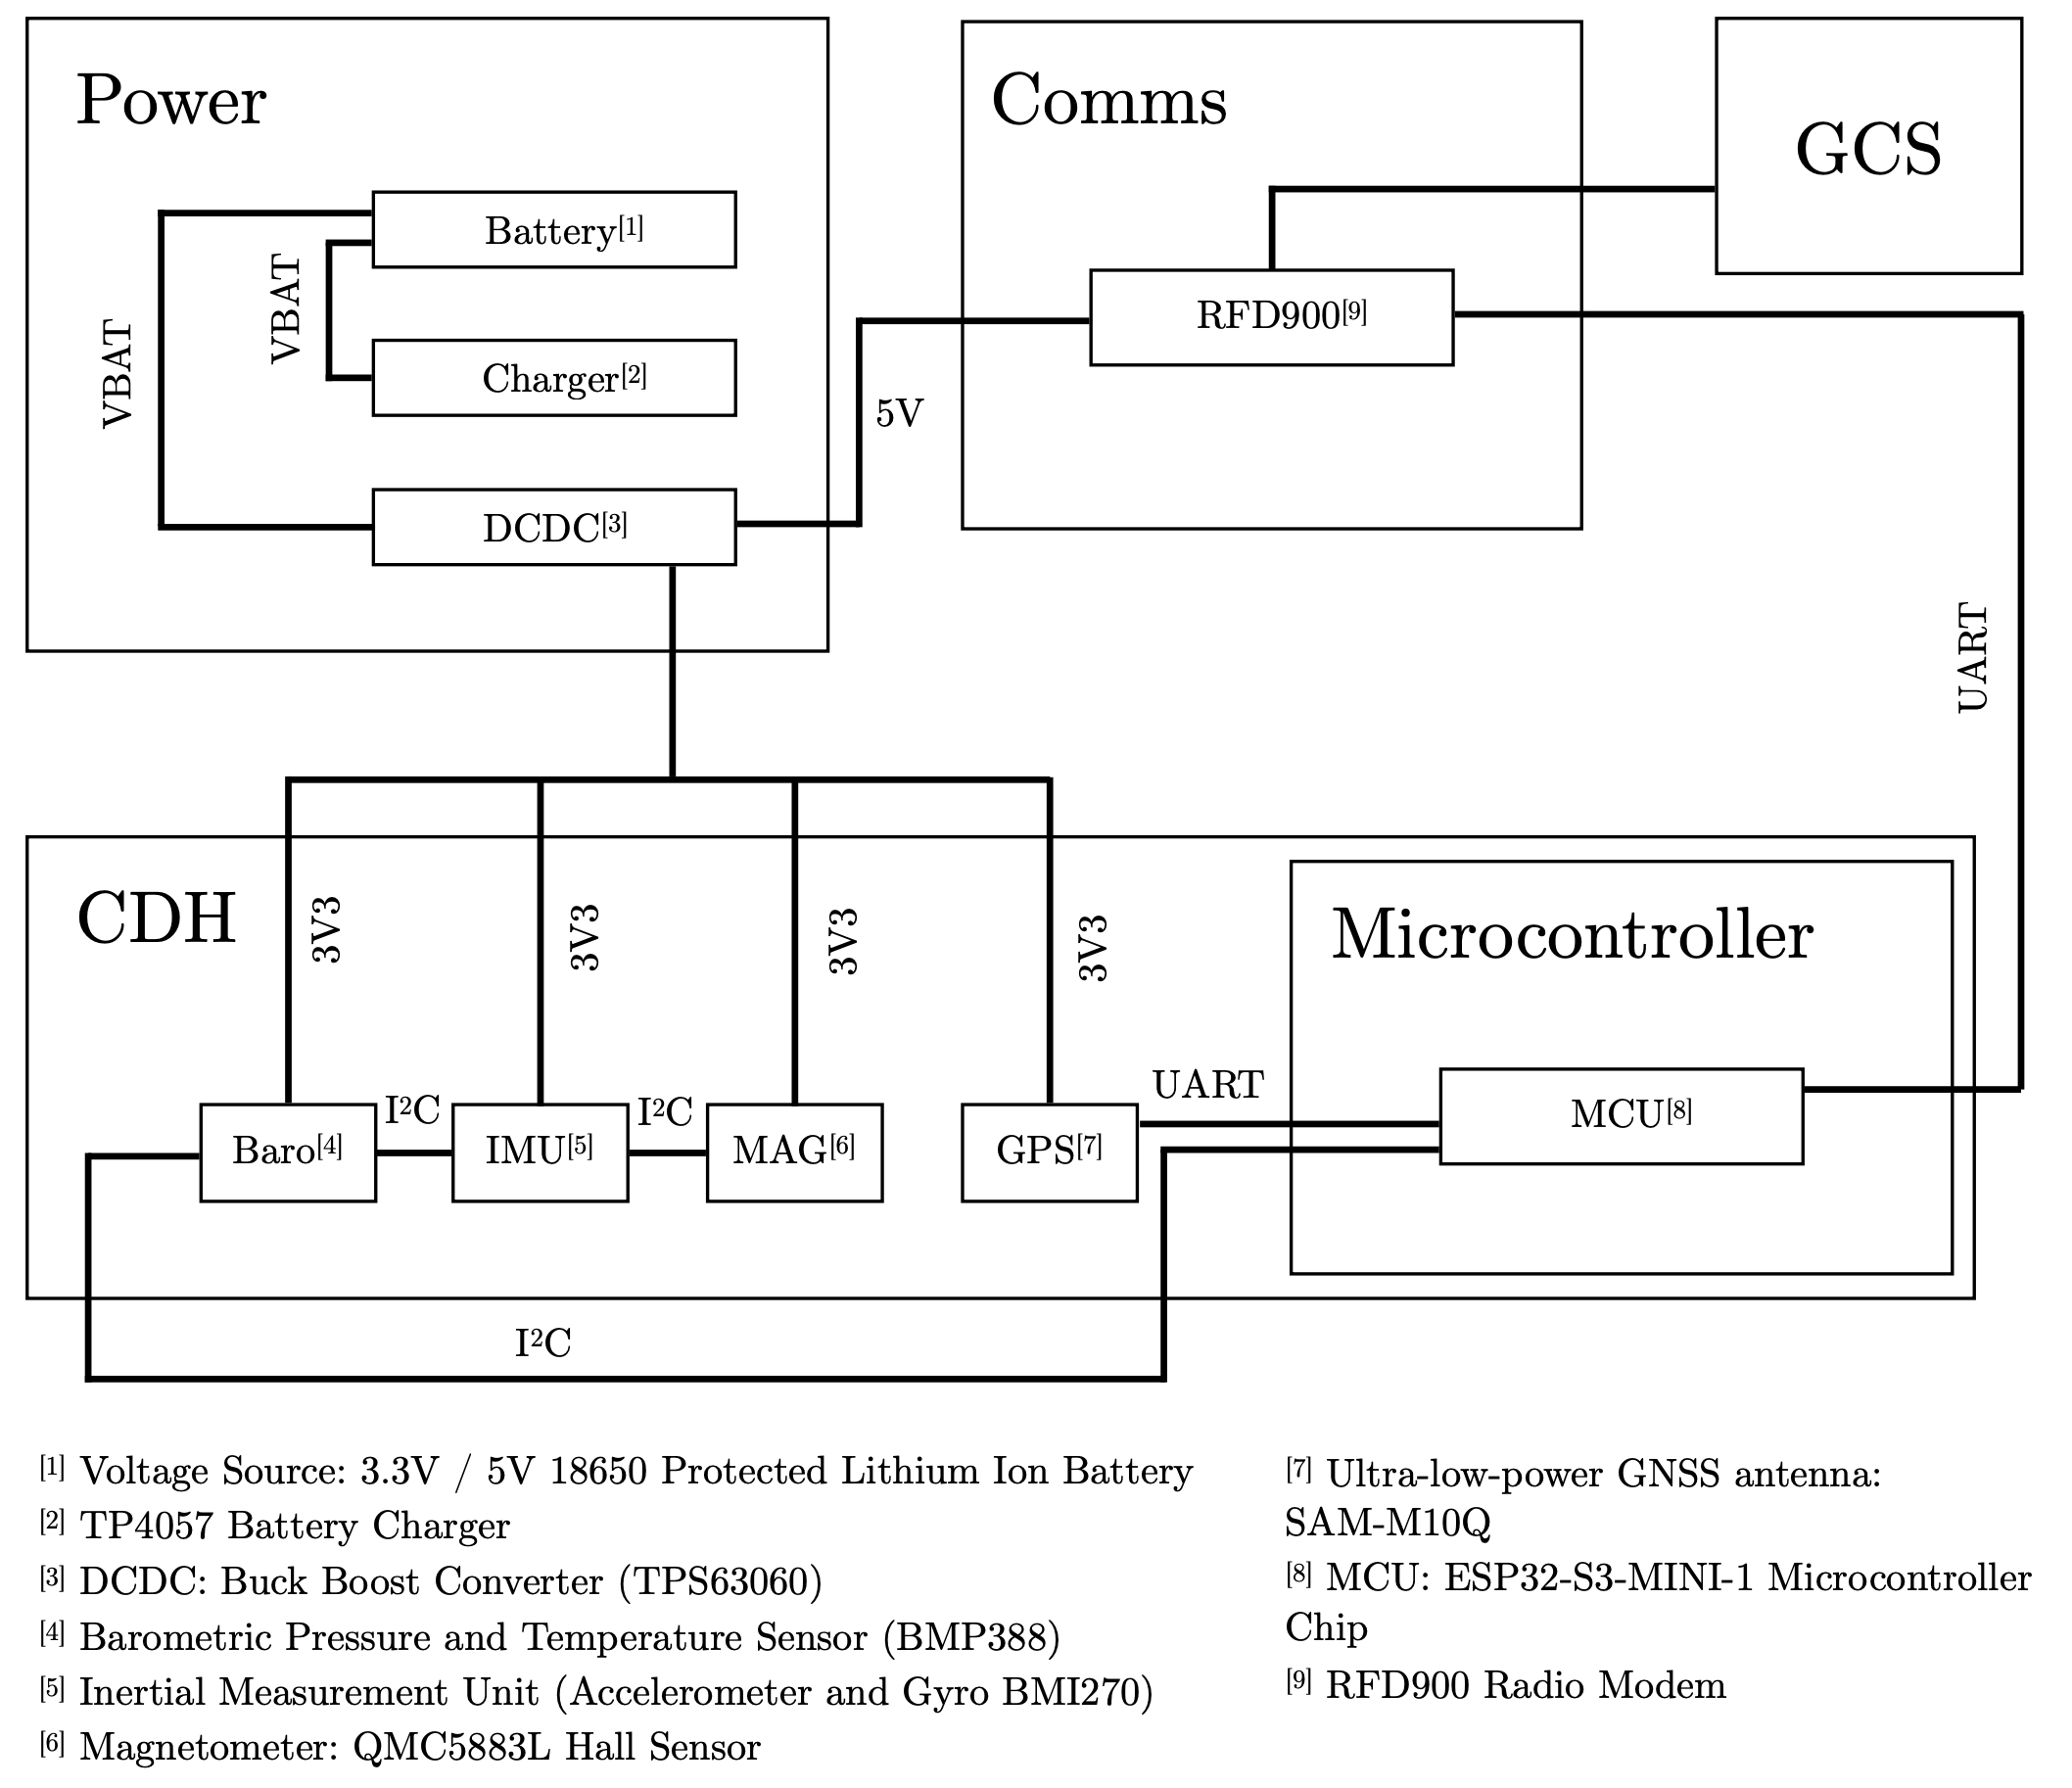
\includegraphics[width=0.8\textwidth]{figures/CUBESAD.png}
                \caption{Block Diagram of the Payload Subsystem}
                \label{fig:payload}
            \end{figure}
            The payload subsystem of the CubeSAT project is essential for the success
            of the project and for the collection of data.
            The system is powered via a 18650 LiPo battery which is regulated to 3.3V 
            to power the barometer, IMU, Magnetometer, GPS, and microncontroller (ESP32-S3-Mini-1).
            The CubeSAT project consists of 5 PCBs with a 3D printed structure to house the components.
            \begin{itemize}
                \item Batteries
                \item Power Regulation
                \item Communication and Data Handling
                \begin{itemize}
                    \item Microcontroller PCB
                    \item Sensor PCB
                    \begin{itemize}
                        \item QMC5883L Magnetometer
                        \item BMI270 IMU
                        \item BMP388 Barometer
                        \item SAM-M10Q GPS
                        \item ESP32-S3-Mini-1
                    \end{itemize}
                \end{itemize}
                \item Communications
                \begin{itemize}
                    \item RFD900
                    \item Antennas
                \end{itemize}
                \item Communication Transmission (Antennae)
            \end{itemize}
            \subsection{Communication and Data Handling}
                \subsubsection{Microcontroller Selection}
                    The microcontroller serves as the central processing unit for the 
                    CDH system, interfacing with sensors and managing data flow.
                    The selection process shall consider the following requirements
                    \begin{itemize}
                        \item Support for I2C, and SPI communication protocols
                        \item Dual-core architecture for efficient multitasking 
                        \item UART/Serial support for programming and communication
                        \item USB bootloader availability for easy firmware updates
                        \item Integrated flash memory for code storage (optional)
                        \item Arduino IDE compatibility for ease of development
                    \end{itemize}
                    By factoring the above requirements, the following options
                    were considered
                    \begin{itemize}
                        \item ESP32-S3-Mini-1
                        \item RP2040
                        \item STM32-F103
                    \end{itemize}
                    Given the similarity in functionality, and development support between
                    all three options, the ESP32-S3-Mini has been chosen for its reliability, 
                    prior experience with the team, and lack of impedance issues present in 
                    options such as the RP2040. Furthermore, its superior performance and efficiency
                    compared to other options make it a viable candidate for future improvements,
                    and enhancements to the project.
                \subsubsection{GPS Selection}
                    The GPS module serves as the primary source of location data for the
                    CubeSAT, providing accurate positioning information for the payload. 
                    The selection process shall consider the following requirements
                    \begin{itemize}
                        \item Accuracy
                        \begin{itemize}
                            \item Support for multi-band GNSS (L1/E1), with a < 1.5m horizontal accuracy
                            \item Position updates at a minimum rate of 10Hz for real-time tracking and navigation
                        \end{itemize}
                        \item Communication
                        \begin{itemize}
                            \item UART communication upto 115200 baud for interfacing with the microcontroller
                            \item Power efficient serial communication operation
                        \end{itemize}
                        \item Operating power
                        \begin{itemize}
                            \item 3.3 or 5V operating voltage for optimal compatibility with existing power systems
                            \item Consumption of $<$ 25mA during continuous tracking to remain within limited power budgets
                        \end{itemize}
                    \end{itemize}
                    Taking into account the above requirements, the SAM-M10Q GPS module was chosen 
                    for its high accuracy, low power consumption, and compatibility with the ESP32-S3-Mini.
                    The module provides a high update rate of 10Hz, and supports multi-band GNSS for
                    improved accuracy and reliability. Furthermore, its low power consumption of 21mA at 3.3V
                    makes it an ideal candidate for the CubeSAT project \cite{sammdatasheet}
                \subsubsection{IMU Trade Study}
                    A low power, high accuracy IMU is essential for the CubeSAT project, providing
                    accurate orientation and motion data for the payload. The selection process shall
                    consider the following requirements
                    \begin{itemize}
                        \item Low cost (less than \$10 per unit)
                        \item Low power and high precision (up to $\pm$ 16g accelerometer, $\pm$ 2000 degree/s gyroscope)
                        \item Flexibility in communication (I2C, SPI)
                    \end{itemize}
                    By factoring the above requirements, the BMI270 IMU was chosen for its high accuracy,
                    low power consumption, and compatibility with the ESP32-S3-Mini. The module provides
                    a wide range of motion sensing capabilities, with a $\pm$ 16g accelerometer, and $\pm$ 2000 $\circ$/s gyroscope.
                    Furthermore, its low power consumption of 700$\mu$A during operation, i2C (up to 3.4MHz) and SPI (up to 10MHz) communication
                    interfaces, dual core architecture with a 16KB FIFO buffer for configuration and buffering,
                    Arduino libraries for easy integration, and low cost of \$7 to \$10 per unit make it an ideal candidate for the CubeSAT project \cite{bmidatasheet}
                \subsubsection{Magnetometer Trade Study}
                    A space, cost, and energy efficient magnetometer is essential for the CubeSAT project,
                    providing accurate magnetic field data for the payload. The selection process shall consider
                    the following requirements
                    \begin{itemize}
                        \item Low cost (less than \$5 per unit)
                        \item Low power and high precision (up to $\pm$ 8 gauss)
                        \item Flexibility in communication (I2C, SPI)
                        \item Small form factor for easy integration
                        \item Wide operating temperature range (-40 to 85 $^\circ$C)
                        \item Low power consumption (less than 100$\mu$A)
                    \end{itemize}
                    By factoring the above requirements, the QMC5883L magnetometer was chosen for its high accuracy,
                    low power consumption, and compatibility with the ESP32-S3-Mini. The module provides a wide range of magnetic field sensing capabilities,
                    with a $\pm$ 8 gauss range, and 0.2 gauss resolution. Furthermore, its low power consumption of 100$\mu$A during operation, I2C (up to 400kHz) communication interface,
                    while it lacks SPI support, its small form factor, wide operating temperature range, and low cost of \$2 to \$5 per unit make it an ideal candidate for the CubeSAT project \cite{qmcdatasheet}
                \subsubsection{Barometer Trade Study}
                    A space, cost, and energy efficient barometer is essential for the CubeSAT project,
                    providing accurate pressure data for the payload. The selection process shall consider
                    the following requirements
                    \begin{itemize}
                        \item Low cost (less than \$5 per unit)
                        \item Wide operating temperature range (-40 to 85 $^\circ$C)
                        \item Wide operating pressure range (30 to 125 kPa)
                        \item High absolute accuracy ($\pm$ 50 Pa)
                    \end{itemize}
                    Three barometers were considered for the CubeSAT project, the ICP10101, S-THP-01A, and
                    the BMP388. However, the BMP388's superior accuracy (50Pa vs 100Pa for the ICP10101),
                    support for a wider range of communication protocols (i2C and SPI vs i2C only for the ICP10101, and 
                    RS485 for the S-THP-01A), and lower cost (\$1.65 for the BMP388 vs \$6.08 for the ICP10101, and \$55.09 for the S-THP-01A)
                    make it an ideal candidate for the CubeSAT project \cite{bmpdatasheet}
            \subsection{Power}
                Power is supplied to the payload system via two 18650 LiPo batteries in parallel.
                The batteries are regulated to 3.3V via a pair of TPS63060DSCR buck-boost converters, regulating
                voltage to 5V and 3.3V for the payload system, with an STC3100IQT battery monitor to monitor battery
                voltage and current.
            \subsection{Radio Modem}
                The RFD900 radio modem is used for communication between the CubeSAT and the ground station.
                The modem operates on the 915MHz frequency band, with a maximum output power of 1W, and a range of up to 40km.
                The modem supports serial communication at up to 115200 baud, with a power consumption of 1.5W during transmission,
                and 0.5W during reception.
                Simple integration using the MAVLink Protocol, and 
                support for AES-128 encryption allows for easy integration and secure communication between the CubeSAT and the ground station.
            \subsection{Antenna}
                The antenna system consists of a pair of dipole antennas, one for the CubeSAT, and one for the ground station.
                The antennas are tuned to the 915MHz frequency band, with a gain of 2.15dBi, and a VSWR of 1.5:1.
                The antennas are connected to the RFD900 radio modem via SMA connectors, providing a reliable and efficient
                communication link between the CubeSAT and the ground station.
    \chapter{Design Implementation}
        \section{Communication PCB Design}
        \section{CDH PCB Design}
        \section{Power PCB Design}
        \section{Data Handling}
            \begin{figure}[H]
                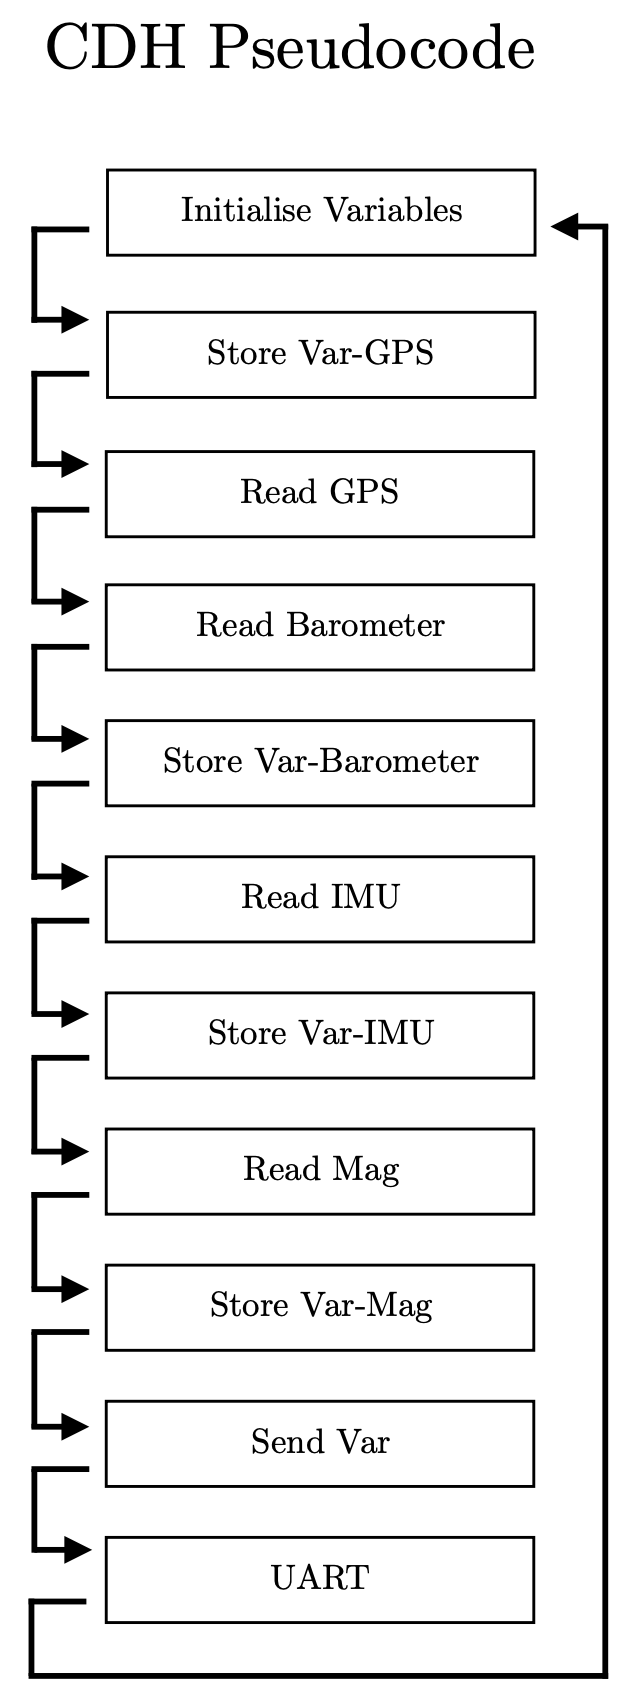
\includegraphics[width=0.8\textwidth]{figures/CDH_CODE.png}
                \caption{Data Handling Program Flowchart}
                \label{fig:cdh}
            \end{figure}
    \chapter{Design Verification and Validation}
        \section{Payload Subsystem}
            \subsection{Microcontroller}
                The data handling code was first tested for functionality
                on a development board before being ported to the 
                ESP32-S3-Mini-1. The code was tested for functionality
                and performance, with the microcontroller interfacing
                with the sensors.
        \chapter{System Requirements Compliance}
    \printbibliography
\end{document}
